\section{La verifica di circuiti digitali}\label{capitolo6}
La verifica di circuiti digitali permette di confrontare due circuiti date le loro specifiche e di dimostrare anche che due specifiche sono equivalenti. Il modo più semplice per verificare l'equivalenza tra due circuiti è quella di sfruttare la rappresentazione tramite \emph{Binary Decision Diagram} (BDD)
\subsection{Binary decision diagram}
Il BDD è una forma di rappresentazione \emph{canonica} delle funzioni logiche che utilizza un grafo per rappresentare tali funzioni, questa metodo permette una rappresentazione compatta delle funzioni ed anche l'analisi su di essa eseguita risultano molto veloci con complessità lineare. Tuttavia, questo grafo può diventare molto grande in base all'ordinamento delle variabili.
Un esempio di BDD è quello mostrato i \figurename\,\ref{fig:bdd} a differenza di un DAG nel caso di BDD vediamo come la dimensione del grafo dipenda solo dai nodi e non dal numero di percorsi possibili.\\
\begin{figure}
\centering
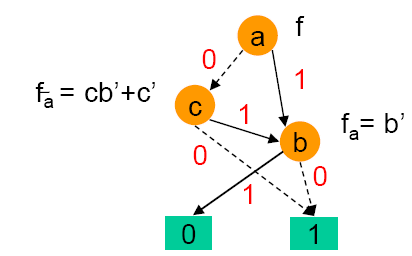
\includegraphics[scale=0.5]{img/bdd.png}
\caption{Esempio di grafo BDD}\label{fig:bdd}
\end{figure}
Un evoluzione del BDD è il ROBDD (\emph{Reduced Ordered Binary Decision Diagram}) ovvero un grafo aciclico con un solo nodo radice e solo due voglie che indicano le uscite \emph{0} e \emph{1} per ogni nodo indiciamo una sola variabile che può avere solamente due figli, inoltre, rispetto ad un normale BDD l'albero è \emph{ridotto} ovvero, un nodo con due figli uguali viene rimosso, due nodi con BDD isometrici vengono uniti. Inoltre il grafo è \emph{ordinato} ovvero i cofattori delle variabili seguono lo stesso ordine durante tutto il percorso, un esempio di BDD ordinato è mostrato in \figurename\,\ref{fig:obdd} nel quale l'ordinamento dei nodi seguito è \emph{a,c,b}.\\
\begin{figure}
\centering
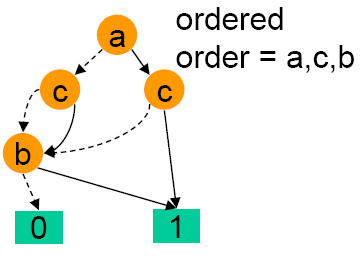
\includegraphics[scale=0.5]{img/obdd.png}
\caption{Esempio di BDD ordinato con ordinamento \emph{a,c,b}}\label{fig:obdd}
\end{figure}
Tuttavia costruire un ROBDD no è molto semplice, fortunatamente ci viene in aiuto la \emph{unique table} una tabella che evita la duplicazione dei nodi esistenti tramite una tabella hash, inoltre tramite una seconda tabella denominata \emph{computed table} si evita il ricalcolo di risultati esistenti.\\
Il BDD non è altro che un albero dei cofattori di Shannon compresso. Quello che fa del ROBDD una forma canonica sono tre fattori fondamentali:
\begin{itemize}
\item Esiste un solo nodo per le costanti "0" e "1"
\item Ordine identico per le variabili lungo percorsi differenti
\item La unique table assicura che:
$$(node(f_{v}=node(g_{v})\wedge (node(f_{\overline{v}})=node(g_{\overline{v}})) \Rightarrow node(f)=node(g)$$
\end{itemize}
Consideriamo ora tre variabili del BDD \emph{f, g, h} e definiamo il costrutto \emph{ite} (\emph{if then ele})
$$
\begin{array}{rcl}
ite(f,g,h) & = & fg+\overline{f}h\\
& = & v(fg+\overline{f}h)_{v}+\overline{v}(fg+\overline{f}h)_{\overline{v}}\\
& = & v(f_{v}g_{v}+\overline{f}_{v}h_{v})+\overline{v}(f_{\overline{v}}g_{\overline{v}}+\overline{f}_{\overline{v}}h_{\overline{v}})\\
& = & ite (v,ite(f_v,g_v,h_v),ite(f_{\overline{v}},g_{\overline{v}},h_{\overline{v}}))\\
& = & v,ite(f_v,g_v,h_v),ite(f_{\overline{v}},g_{\overline{v}},h_{\overline{v}})
\end{array}
$$
Dove \emph{v} p la variabile più in alto dell'BDD formato da \emph{f, g, h}.
Tramite l'operatore \emph{ite} possiamo implementare fino a 16 funzioni logiche di due variabili come mostrato in \figurename\,\ref{fig:itefun}.\\
\begin{figure}
\centering
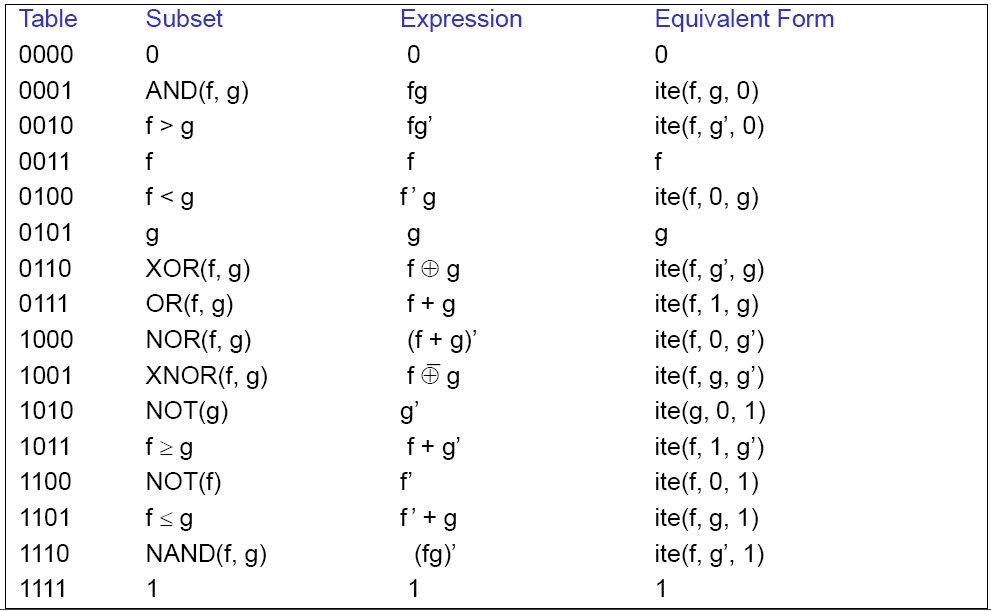
\includegraphics[scale=0.5]{img/itefun.png}
\caption{Equivalente \emph{ite} delle funzioni logiche più comuni}\label{fig:itefun}
\end{figure}
Un ottimizzazione di questa tecnica prevede l'utilizzo degli \emph{archi complementari} che permette di ridurre l'utilizzo di memoria e migliora le prestazioni di alcune operazioni.
tuttavia per mantenere la forma canonica dobbiamo effettuare quattro equivalenze mostrate in \figurename\,\ref{fig:complementedge}.\\
\begin{figure}
\centering
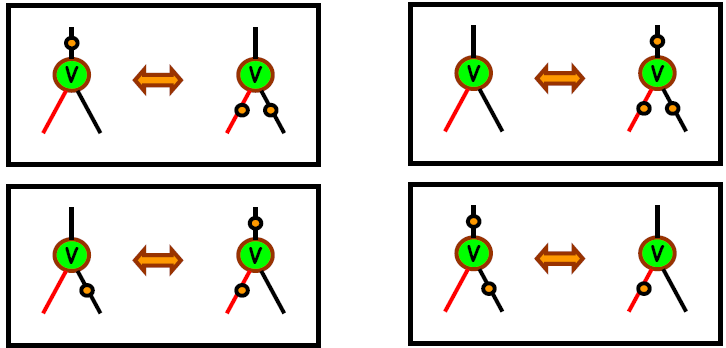
\includegraphics[scale=0.5]{img/complementedge.png}
\caption{Equivalenze nell'utilizzo degli archi complementari.}\label{fig:complementedge}
\end{figure}
Un aspetto importante nell'utilizzo del BDD è il rilascio della memoria non più utilizzata dai nodi, tale rilascio deve essere effettuato tramite la chiamata della funzione \texttt{bdd\_free}. Esistono due meccanismi per verificare se un nodo non è più referenziato, il primo prevede un \emph{reference counter} su ogni nodo che tiene traccia dei riferimenti ancora attivi, il contatore è incrementato quando un nuovo riferimento viene creato, mentre viene decrementato quando il nodo viene deferenziato. Il secondo meccanismo denominato \emph{mark and sweep} non necessita di contatori, in una prima fase si marcano tutti i nodi del BDD che sono referenziati, in una seconda fase si rimuovono quelli che non sono marcati.\\
Un'altra caratteristica importante per il garbage collector è quello del time in quanto l'operazione è molto costosa; si potrebbe pensare a eliminare i nodi non appena questi vengono rilasciati, tuttavia in molti casi non è conveniente in quanto alcuni nodi vengono referenziati nell'istruzione successiva, in realtà si utilizzano dei garbage collector basati su statistiche raccolte durante l'esecuzione. Un altro aspetto da considerare è la \emph{computed table} che deve essere svuotata da quei valori che comprendono nodi non più referenziati.\\
Dal BDD negli anni ci si è evoluti in meccanismi in po più sofisticati:
\begin{description}
\item[MDD:] \emph{Multi-Valued} BDD è un BDD con più di due archi uscenti
\item[ADD:] \emph{Analog} BDD l'albero delle decisioni questa volta prevede anche numeri reali e non solo 0,1
\end{description}
Una delle varianti del BDD più utilizzata è la \emph{zero suppressed BDD} nel quale si eliminano i nodi nei quali l'arco then punta a 0 e si connette l'arco entrante al ramo dell'else.
\subsection{Diagramma And-Inverter}
Il grafico \emph{and-inverter} è un grafico che utilizza solamente \texttt{and} con due ingressi e \texttt{inverter} sugli archi per rappresentare un qualsiasi circuito, un esempio di tale traduzione è mostrato in \figurename\,\ref{fig:andinverter}.\\
\begin{figure}
\centering
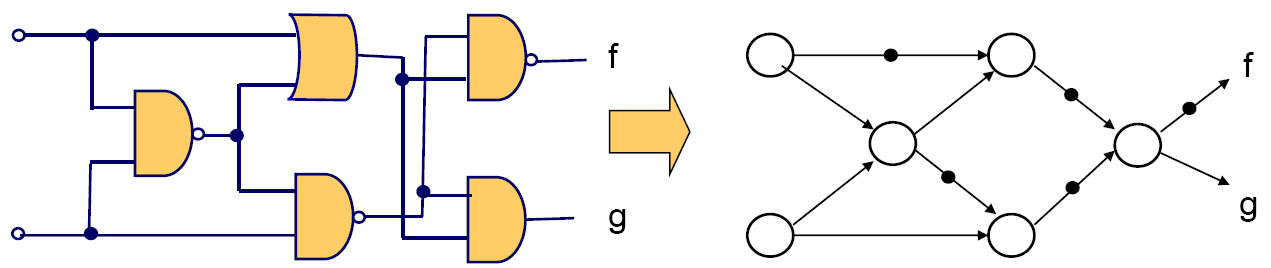
\includegraphics[scale=0.5]{img/andinverter.png}
\caption{Esempio di conversione di un circuito in forma \emph{and-inverter}}\label{fig:andinverter}
\end{figure}
Dato il grafico and-inverter si possono applicare alcuni algoritmi per studiare alcuni aspetti del circuito, come l'equivalenza rispetto ad un altro o anche per la generazione di vettori di test. Uno di questi algoritmi è il SAT il quale prevede l'assegamento a 1 dell'uscita per calcolarne i valori degli ingressi. Una implementazione di questo algoritmo è la \emph{Davis-Putnam Procedure} nella quale si ricercano degli assegnamenti per l'intero cono di archi che arrivano ad un determinato vertice tramite un meccanismo di prove su tutte le combinazioni. Si mantiene una coda dei vertici da giustificare, si preleva il vertice richiesto dalla coda e si effettua un case split dei possibili assegnamenti. Per ogni caso si effettua la propagazioni tramite le implicazioni possibili, nel caso vi siano vertici da giustificare si aggiungono alla coda, in caso di conflitto si disfano le implicazione e si prova un altro caso fino a svuotare la coda dei vertici.\\
Il segreto di un risolutore SAT efficente è una veloce procedura delle implicazioni. In questo caso abbiamo 27 possibili casi come mostrato in \figurename\,\ref{fig:satimp} di cui solo l'ultima genera l'introduzione di un nuovo nodo nella coda dei \emph{case split}.
\begin{figure}
\centering
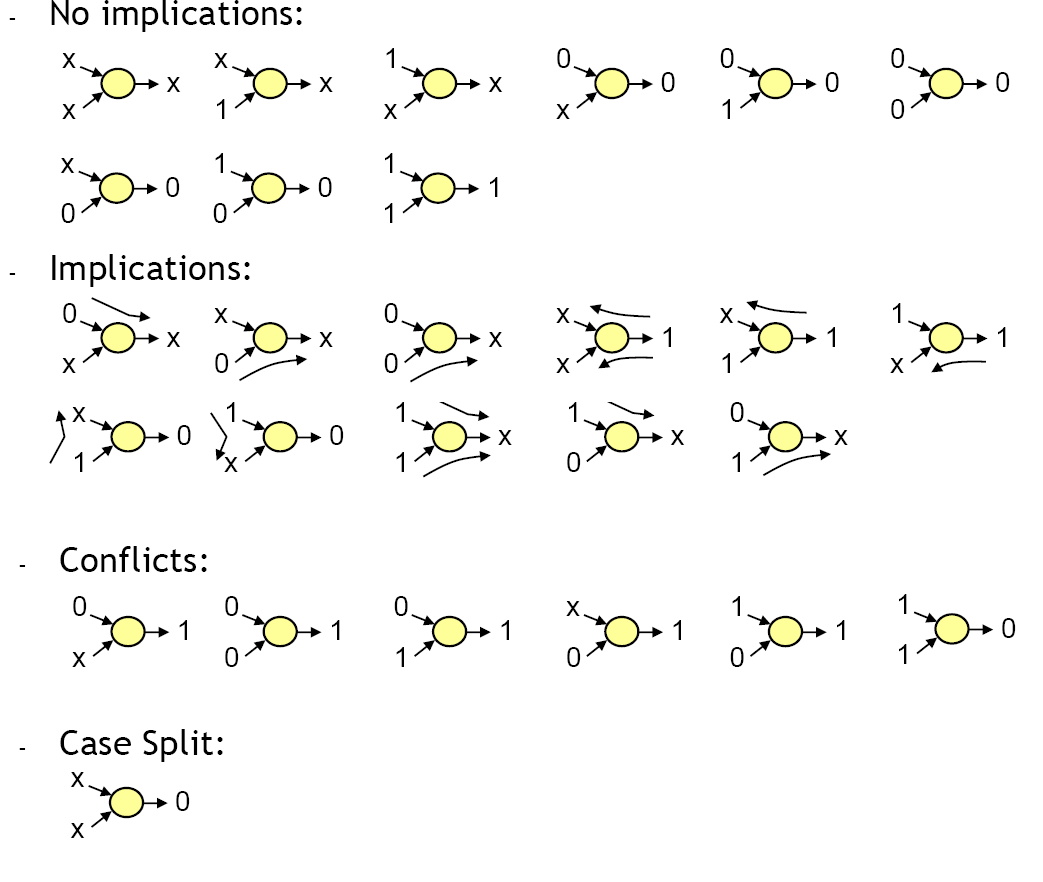
\includegraphics[scale=0.4]{img/satimp.png}
\caption{Possibili implicazioni nel meccanismo sat}\label{fig:satimp}
\end{figure}
Un esempio di questo algoritmo è mostrato in \figurename\,\ref{fig:satexemp}
\begin{figure}
\centering
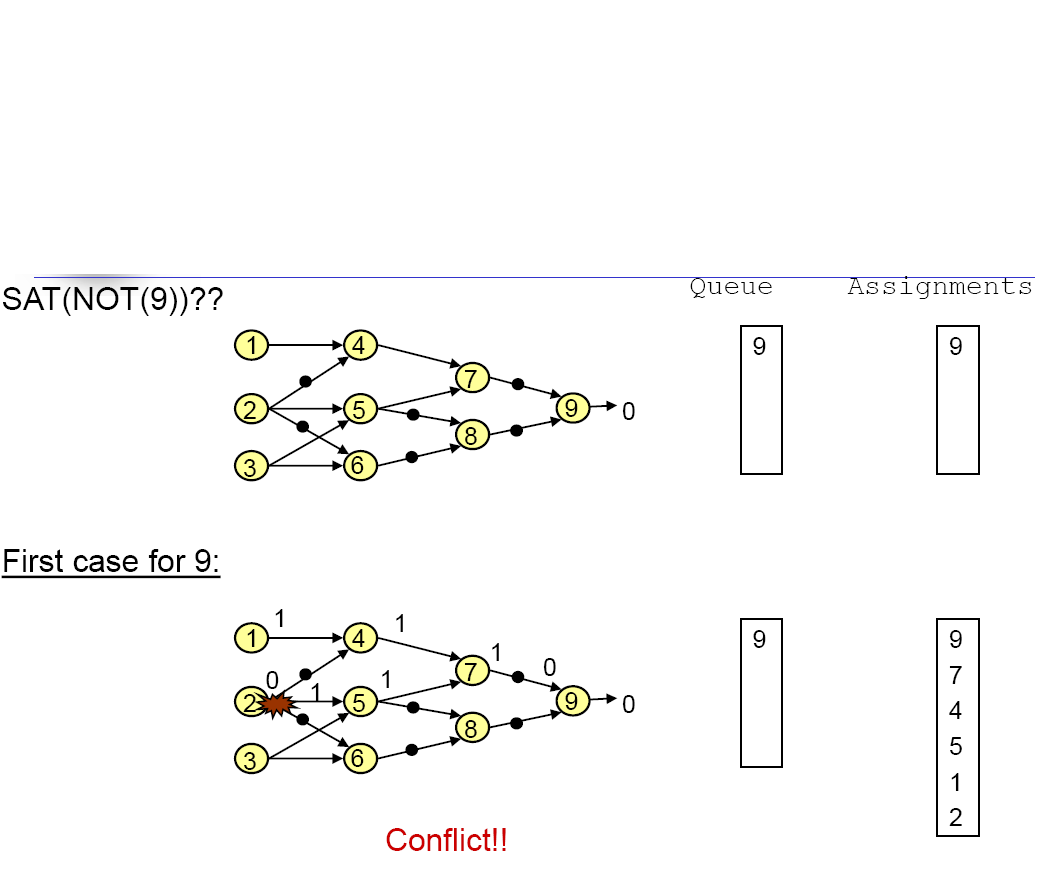
\includegraphics[scale=0.5]{img/satexemp.png}
\caption{Esempio di algoritmo SAT}\label{fig:satexemp}
\end{figure}
\subsubsection{Learning}
I meccanismi di learning sono meccanismi che introducono delle scorciatoie nel circuito per minimizzare i possibili case split e velocizzare gli algoritmi. Esistono meccanismi di \emph{static learning} che controllano le implicazioni su tutto il circuito e meccanismi di \emph{dynamic learning} che invece controllano solo la sezione in analisi.\\
Un meccanismo di learning ad esempio nella prima fase dell'esempio precedente la quale generava un conflitto sul vertice 7 potrebbe prevedere di assegnare quel vertice a 0 visto che l'assegnamento ad 1 provoca un conflitto come mostrato in \figurename\,\ref{fig:firstlearning}.\\
\begin{figure}
\centering
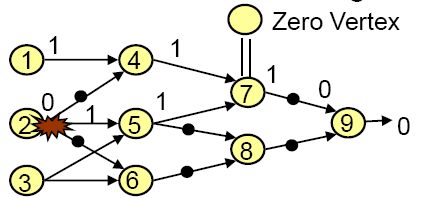
\includegraphics[scale=0.6]{img/firstlearning.png}
\caption{Esempio di dynamic learning}\label{fig:firstlearning}
\end{figure}
Un esempio di \emph{static learning} invece prevede il riconoscimento di pattern predefiniti come i due in \figurename\,\ref{fig:static1} e \ref{fig:static2} che possono essere sostituiti come nelle figure.
\begin{figure}
\subfigure[]{
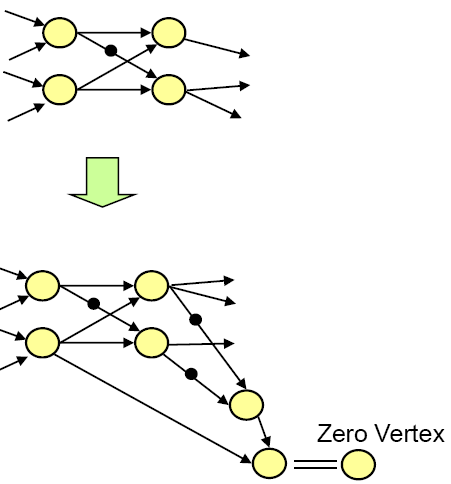
\includegraphics[scale=0.5]{img/static1.png}
\label{fig:static1}
}
\subfigure[]{
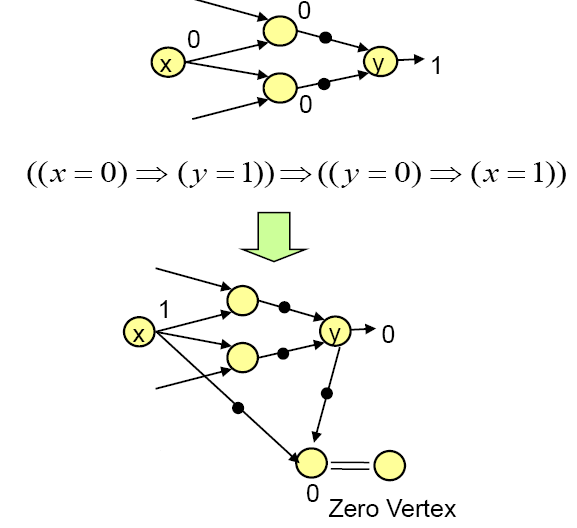
\includegraphics[scale=0.5]{img/static2.png}
\label{fig:static2}
}
\end{figure}
\subsection{BDD Swepping}
Il BDD swepping è un algoritmo che combina diverse tecniche per migliorare le performance dell'analisi, in particolare questo algoritmo sfrutta l'and-inverter graph per modellare il circuito e la propagazione BDD per migliorare il calcolo delle priorità dei nodi. Per un esempio rimandiamo alle slide del corso.
\subsection{Equivalece checking}